\documentclass[12pt]{report}
\usepackage[top = 0.75 in]{geometry}
\usepackage[bottom]{footmisc}
\usepackage[]{geometry}
\usepackage{graphicx}
\usepackage{amsmath}
\usepackage{longtable}
\usepackage{enumerate}
\usepackage{changepage}
\usepackage{caption}
\usepackage{amsmath}

\newcommand{\mychapter}[2]{
    \setcounter{chapter}{#1}
    \setcounter{section}{0}
    \chapter*{#2}
    \addcontentsline{toc}{chapter}{#2}
}
\usepackage[tableposition=top]{caption}

\begin{document}
  \title{
   \ Kwame Nkrumah Univeristy of Science and Technology, Kumasi, Ghana.\\
   { \huge COE 381: Microprocessors}\\
   \begin{center}
    
\includegraphics[scale=0.9]{knust-logo}
    \end{center}
    Design and Simulation of a Single Cycle 32 bit MIPS Reduced Instruction Set CPU Using Logisim}
    \author{ Computer Engineering 3\\ Group 1}
    \maketitle
    \begin{center}
    \begin{table}{}
    {\centering \Huge Group Members}\\
     \renewcommand{\arraystretch}{2}
   \begin{tabular}{|p{7cm}|p{3cm}|p{4cm}|}
     \hline
    {\Large \textbf{Name}}&{\Large \textbf{Index Number}}&\textbf{\Large Signature}\\\hline
    {\large Kumbong Hermann Nyuykonge}& {\large 5952816}&\\\hline
    {\large Atuobi Alexander }&{\large 5948316}&\\\hline
    {\large Oluwatobi Mathieu Boko}&{\large 5949516}&\\\hline
    {\large Kudom-Agyemang Emmanuel}&{\large 5952716}&\\\hline
    {\large Kurmodzie Kofi Shim}&{\large 5952916}&\\\hline
    {\large Arthur Hilda}&{\large 5947216}&\\\hline
    {\Large Eric Ndacyayisenga}&{\large 5950816}&\\\hline
   \end{tabular}
    \end{table}
    \end{center}
   \begin{center}
   {\Huge Teamwork and Participation}
\end{center} 
%\begin{center}
    The team met for 6 hours each week to complete the project. All members of the team were present during each session. The order of this document shows the chronology in which we  incrementally built our processor. After discussing the general architecture overview, each member implemented a specific portion of the CPU and we discussed the implementation as a team. We finally combined the implementations into a working CPU as a team.  
    %\end{center}
       \begin{center} \Large Meeting Days\end{center}
   \begin{longtable}{|p{5cm}|p{5cm}|}
     \hline
    {\Large Day}&{\Large Period}\\\hline
    {\large Monday}& {\large 12:00 pm - 2:00 pm}\\\hline
    {\large Tuesday}&{\large 2:00 pm - 4:00 pm}\\\hline
    {\large Thursday}&{\large 2:00 pm - 4:00 pm}\\\hline
   \end{longtable}
   \begin{center}\Large Task Distribution for Implementation\end{center}
    \begin{longtable}{|p{5cm}|p{10cm}|}
     \hline
    {\Large Unit}&{\Large Implementer}\\\hline
    {\large ALU}& {\large Hilda Arthur}\\\hline
    {\large Register File}&{\large Shim Kofi and Eric Ndacyayisenga}\\\hline
    {\large Datapath}&{\large Kumbong Hermann and Oluwatobi Boko}\\\hline
    {\large Control Unit}&{\large Kudom-Agyemang and Atuobi Alexander}\\\hline
   \end{longtable}
    \tableofcontents
    \listoftables
    \listoffigures
    
    \newpage
\renewcommand*\thesection{\arabic{section}}
   \mychapter{1}{The MIPS Instruction Set Architecture}
   \section{Introduction}
   This section is meant to acquaint the reader with the MIPS ISA. A reader familiar with MIPS may jump straight to the next chapter on register design. 
   
   An instruction set architecture (ISA) is an abstract model of a computer. It is also referred to as architecture or computer architecture. A realization of an ISA is called an implementation. An ISA permits multiple implementations that may vary in performance, physical size, and monetary cost (among other things); because the ISA serves as the interface between software and hardware. Software that has been written for an ISA can run on different implementations of the same ISA. This has enabled binary compatibility between different generations of computers to be easily achieved, and the development of computer families. Both of these developments have helped to lower the cost of computers and to increase their applicability. For these reasons, the ISA is one of the most important abstractions in computing today.

An ISA defines everything a machine language programmer needs to know in order to program a computer. What an ISA defines differs between ISAs; in general, ISAs define the supported data types, what state there is (such as the main memory and registers) and their semantics (such as the memory consistency and addressing modes), the instruction set (the set of machine instructions that comprises a computer's machine language), and the input/output model.

The ISA serves as the boundary between software and hardware. We will briefly describe the instruction sets found in many of the microprocessors used today. The ISA of a processor can be described using 5 catagories:
\begin{enumerate}
\item \textbf{Operand Storage in the CPU}\\
Where are the operands kept other than in memory?
\item \textbf{Number of explicit named operands}
How many operands are named in a typical instruction.
\item \textbf{Operand location}
Can any ALU instruction operand be located in memory? Or must all operands be kept internaly in the CPU?
\item \textbf{Operations}
What operations are provided in the ISA.
\item \textbf{Type and size of operands}
What is the type and size of each operand and how is it specified?
\end{enumerate}
Of all the above the most distinguishing factor is the first. 

\section{Classification of Instruction Set Architectures}
 \subsection{Based on operand storage in CPU}
 The 3 most common types of ISAs are:
\begin{enumerate}
\item \textbf{Stack} - The operands are implicitly on top of the stack.
Promoted in the 60’s; limited popularity: Burroughs B5500/6500, HP
3000/70, Java VM

\textbf{Advantages:} Simple Model of expression evaluation (reverse polish). Short instructions.

\textbf{Disadvantages:} A stack can't be randomly accessed This makes it hard to generate eficient code. The stack itself is accessed every operation and becomes a bottleneck.

\item \textbf{Accumulator} - One operand is implicitly the accumulator.
The most popular early architecture: IBM 7090, DEC PDP-8, MOS 6502

\textbf{Advantages:} Short instructions.
 
\textbf{Disadvantages:} The accumulator is only temporary storage so memory traffic is the highest for this approach.

\item \textbf{General Purpose Register (GPR)} - All operands are explicitely mentioned, they are either registers or memory locations
The dominant architecture: CDC 6600, IBM
360/370 (RX), PDP-11, 68000, all RISC
machines, etc.

\textbf{Advantages:} Makes code generation easy. Data can be stored for long periods in registers.

\textbf{Disadvantages:} All operands must be named leading to longer instructions.
\end{enumerate} 

Not all processors can be neatly tagged into one of the above catagories. The i8086 has many instructions that use implicit operands although it has a general register set. The i8051 is another example, it has 4 banks of GPRs but most instructions must have the A register as one of its operands. Earlier CPUs were of the first 2 types but in the last 15 years all CPUs made are GPR processors. The 2 major reasons are that registers are faster than memory, the more data that can be kept internaly in the CPU the faster the program wil run. The other reason is that registers are easier for a compiler to use.

\subsection{Based on architectural complexity}
Based on architectural complexity we can classify ISA's as \textbf{RISC (Reduced instruction set computing)} and \textbf{CISC (Complex instruction set computing)}. CISC has the ability to execute addressing modes or multi-step operations within one instruction set. It  is the design of the CPU where one instruction performs many low-level operations. For example,  memory storage, an  arithmetic operation and loading from memory. RISC  is a CPU design strategy based on the insight that simplified instruction set gives higher performance when combined with a microprocessor architecture which has the ability to execute the instructions by using some microprocessor cycles per instruction.

\begin{enumerate}
\item \textbf{CISC Architecture}

The CISC approach attempts to minimize the number of instructions per program, sacrificing the number of cycles per instruction. Computers based on the CISC architecture are designed to decrease the memory cost. Because, the large programs need more storage, thus increasing the memory cost and large memory becomes more expensive. To solve these problems, the number of instructions per program can be reduced by embedding the number of operations in a single instruction, thereby making the instructions more complex. Examples of CISC processors are : 
IBM 370/168,VAX 11/780 and Intel 80x86 


\textbf{Characteristics of CISC architecture}
\begin{itemize}
\item Instruction-decoding logic will be Complex.
\item One instruction is required to support multiple addressing modes.
\item Less chip space is enough for general purpose registers for the instructions that are 0operated directly on memory.
\item Various CISC designs are set up two special registers for the stack pointer, handling interrupts,  etc.
\end{itemize}

\item \textbf{RISC Architecture}

RISC (Reduced Instruction Set Computer) is used in portable devices due to its power efficiency. For Example, Apple iPod and Nintendo DS. RISC is a type of microprocessor architecture that uses highly-optimized set of instructions. RISC does the opposite, reducing the cycles per instruction at the cost of the number of instructions per program Pipelining is one of the unique feature of RISC. It is performed by overlapping the execution of several instructions in a pipeline fashion. It has a high performance advantage over CISC.RISC processors take simple instructions and are executed within a clock cycle. Examples of RISC families include: DEC Alpha, AMD 29k, ARC, Atmel AVR, Blackfin, Intel i860 and i960, MIPS, Motorola 88000, PA-RISC

\textbf{RISC architecture characteristics}
\begin{itemize}
\item Simple Instructions are used in RISC architecture.
\item RISC helps and supports few simple data types and synthesizes complex data types.
\item RISC utilizes simple addressing modes and fixed length instructions for pipelining.
\item RISC permits any register to be used in any context. However it is usual to use the register in accordance with specified conventions.
\item In RISC, more RAM is required to store assembly level instructions.
Reduced instructions need a less number of transistors in RISC. Table \ref{tab:mips_vs_cisc} presents a comparison of the MIPS and CISC architectures.
\end{itemize}
\end{enumerate}
\begin{longtable}{|p{7cm}|p{7cm}|}
\caption{Comparison of MIPS and CISC architectures}  \label{tab:mips_vs_cisc} \\
\hline
RISC&CISC\\\hline
 RISC stands for Reduced Instruction Set Computer.&CISC stands for Complex Instruction Set Computer.\\\hline
 RISC processors have simple instructions taking about one clock cycle. The average clock cycle per instruction (CPI) is 1.5& CSIC processor has complex instructions that take up multiple clocks for execution. The average clock cycle per instruction (CPI) is in the range of 2 and 15.\\\hline
 Performance is optimized with more focus on software& Performance is optimized with more focus on hardware.\\\hline
 It has no memory unit and uses a separate hardware to implement instructions&It has a memory unit to implement complex instructions.\\\hline
 RISC processors are highly pipelined & They are normally not pipelined or less pipelined\\\hline
Decoding of instructions is simple.&Decoding of instructions is complex\\\hline
The most common RISC microprocessors are Alpha, ARC, ARM, AVR, MIPS, PA-RISC, PIC, Power Architecture, and SPARC & Examples of CISC processors are the System/360, VAX, PDP-11, Motorola 68000 family, AMD and Intel x86 CPUs.\\\hline
\end{longtable}
Other types include very long instruction word (VLIW) architectures, and the closely related long instruction word (LIW) and explicitly parallel instruction computing (EPIC) architectures. These architectures seek to exploit instruction-level parallelism with less hardware than RISC and CISC by making the compiler responsible for instruction issue and scheduling.

Architectures with even less complexity have been studied, such as the minimal instruction set computer (MISC) and one instruction set computer (OISC). These are theoretically important types, but have not been commercialized.

\section{MIPS ISA}
   MIPS stands for \textbf{Microprocessor without interlocked pipeline stages.} It is a reduced instruction set computer (RISC) instruction set architecture (ISA) developed by MIPS technologies. The most recent version of MIPS is MIPS32/64 Release 6.\footnote{As of the time of writing this paper}. The MIPS architecture grew out of an early 1980's research project at Stanford University. In
1984, MIPS computer corporation was founded to commercialize this research. However, CPU
chips based on the MIPS architecture have been produced by a number of different companies,
including LSI Logic, Toshiba, Philips, NEC, IDT, and NKK. Though the architecture is a
quarter of a century old, MIPS-architecture chips are widely used in current systems such as
CISCO Routers, TiVo Series 2 and many other embedded applications including set-top boxes
for digital TV, cable modems, DVD recorders, and printers. We use it in this project, because of
its clean and simple architecture.

The MIPS ISA is built on 3 major design principles
\begin{enumerate}[i]
\item \textbf{Simplicity favors regularity}
\item \textbf{Smaller is faster}
\item \textbf{Good design demands good compromises}
\end{enumerate}
The MIPS architecture itself has passed through a series of evolutions, starting with MIPS I and then evolving into MIPS
II, MIPS III, and MIPS IV. Each successive ISA is a superset of the preceding one - so anything
found in MIPS I is also found in MIPS II, III, and IV, etc. The MIPS I and II ISA's were 32 bit
architectures. MIPS III added 64 bit capabilities - but with the core 32 bit architecture as a
subset, and MIPS IV expanded on this. This project deals only with a subset of the core MIPS
I architecture.

   
Although MIPS is a RISC ISA providing a complete description is a tedious task that we will not concern ourselves with here. We provide a brief summary rather than an exhaustive coverage of MIPS in the section that follows. Interested readers may ferret online resources for  a more thorough coverage of the topic. The material covered below will however be enough to follow the remainder of this paper.

The MIPS-32 has a 32 bit architecture, with 32 bit instructions, a 32
bit data word, and 32 bit addresses.
It has 32 addressable internal registers requiring a 5 bit register address.
Register 0 always has the the constant value 0.
Addresses are for individual bytes (8 bits) but instructions must have
addresses which are a multiple of 4(instructions
must be word aligned in memory).

\section{MIPS Instruction formats}
There are three basic instruction types with the following formats:
\begin{enumerate}
 \item \textbf{R-Type Instructions}
 
 Arithmetic, logical, and shift-type operations are performed on MIPS using R-Type(register) instructions,
which encode the operation to be performed and three general registers (two sources and a
destination). Shift instructions may also encode the number of places to shift. It is conventional,
in MIPS documentation, to refer to the two source registers as rs and rt, and the destination
register as rd. Each of these is actually encoded in the instruction as a 5-bit integer that specifies
one of the 32 general registers. In assembly language, the registers can be specified by using
their generic names (e.g. \$8) or their special names (e.g. t0).

\begin{center}
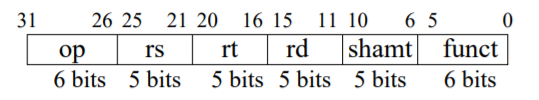
\includegraphics[scale=1]{R-type}\\
R-Type instruction format
\end{center}

For all R-type instructions, the op field is 000000.
The \textit{funct} field selects the particular type of operation for R-type
operations.
The \textit{shamt} field determines the number of bits to be shifted (0 to
31).
These instructions perform the following:

\begin{equation*}
R[rd] \leftarrow R[rs] ~~~op~~~ R[rt]
\end{equation*}

\begin{longtable}{|p{4cm}|p{5cm}|p{5cm}|}
\caption{Examples of R-Type Instructions} \label{tab:examples_r_type} \\
\hline
Instruction &Example&Meaning\\\hline
\texttt{add}&\texttt{add \$s1, \$s2, \$s3 }&\texttt{ \$s1 = \$s2 + \$s3}\\\hline
\texttt{subtract}&\texttt{sub \$s1, \$s2, \$s3}&\texttt{ \$s1 = \$s2 - \$s3}\\\hline 
\texttt{and}&\texttt{and \$s1, \$s2, \$s3 }&\texttt{ \$s1 = \$s2 ~\&~ \$s3}\\\hline
\end{longtable}

 \item \textbf{I-Type Instructions}
 
 For certain operations, it is also possible to specify a constant as one of the two operands. The
constant is coded into the instruction as a 16-bit integer; therefore, it must lie in the range
$-32678 \leq constant \leq 32767$ (for addi, addiu, slti, sltiu) or $0 \leq constant \leq 65535$ (for andi,
ori, xori). The constant is turned into a 32-bit value either by filling the upper 16 bits with a
copy of the sign bit (addi, addiu, slti, sltiu) or with 0’s (andi, ori, xori). [Note that even
the “unsigned” instructions sign-extend the immediate value!] (For larger constants, it is
necessary to use several instructions).
These instructions perform the following:
\begin{equation*}
R[rt] \leftarrow R[rs] ~~~op~~~ imm
\end{equation*}

\begin{center}
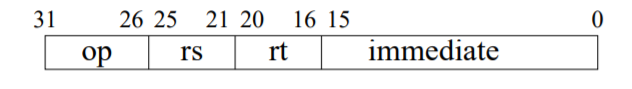
\includegraphics[scale=1]{I-type}\\
I-type instruction format
\end{center}

\begin{longtable}{|p{4cm}|p{5cm}|p{5cm}|}
\caption{Examples of I-Type Instructions} \label{tab:examples_i_type} \\
\hline
Instruction &Example&Meaning\\\hline
\texttt{addi}&\texttt{addi \$s1, \$s2, imm }&\texttt{ \$s1 = \$s2 + imm}\\\hline
\texttt{and}&\texttt{andi \$s1, \$s2, imm }&\texttt{ \$s1 = \$s2 $~\&~$ imm}\\\hline
\texttt{or}&\texttt{ori \$s1, \$s2, imm }&\texttt{ \$s1 = \$s2 $~\vert~$ imm}\\\hline
\texttt{set less than immediate}&\texttt{ slti \$s1, \$s2, imm}&\texttt{if (\$s2 < imm), \$s1=1;
 else \$s1=0}\\\hline
 \texttt{load word}&\texttt{lw \$s1, imm(\$s2)}&\texttt{\$s1 = Memory[\$s2 + imm]}\\\hline
 \texttt{store word}&\texttt{sw \$s1, imm(\$s2)}&\texttt{Memory[\$s2 + imm] = \$s1}\\\hline
\end{longtable}

There is no \textit{subi}. One can subtract a constant by using \textit{addi} with a negative value. 
The standard way to load a (small enough) constant value into a register is to use either
the \textit{addi} or the \textit{ori} instruction with \$0 as the register source.

\textit{load word} and \textit{store word} are the only instructions that access
memory directly.
Because data must be explicitly loaded before it is operated on, and
explicitly stored afterwards, the MIPS is said to be a load/store
architecture.
This is often considered to be an essential feature of a reduced instruction
set architecture (RISC).

Another group of the I-type instructions are the branch instructions as shown in table \ref{tab:examples_c_i_type}. 

\begin{longtable}{|p{3.5cm}|p{3.5cm}|p{7cm}|}
\caption{Examples of I-type Conditional Branch Instructions} \label{tab:examples_c_i_type}\\
\hline
Instruction &Example&Meaning\\\hline
\texttt{branch on equal }&\texttt{beq \$s1, \$s2, imm }&\texttt{\shortstack{if \$s1 == \$s2 \\ go to PC + 4 +(4 $\times$ imm)}}\\\hline
\texttt{branch on not equal}&\texttt{bneq \$s1, \$s2, imm }&\texttt{\shortstack{if \$s1 != \$s2 \\ go to PC + 4 +(4 $\times$ imm)}}\\\hline
\end{longtable}

\item \textbf{J-Type Instructions}
The J-type instructions are all jump instructions.The MIPS processor addresses data at the byte level, but
instructions are addressed at the word level.
Moreover, all instructions must be aligned on a word boundary (an
integer multiple of 4 bytes).
Therefore, the next instruction is 4 byte addresses from the current
instruction.
Since jumps must have an instruction as target, shifting the target
address by 2 bits (which is the same as multiplying by 4) allows the
instruction to specify larger jumps.
Note that the jump instruction cannot span (jump across) all of
memory.

\begin{center}
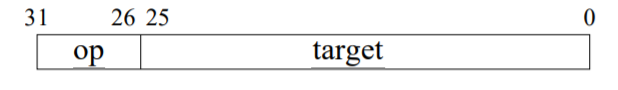
\includegraphics[scale=1]{J-type}\\
J-Type Instruction format
\end{center}

\begin{center}
\begin{longtable}{|p{3.5cm}|p{3.5cm}|p{6cm}|}
\caption{Examples of J-Type Instructions} \label{tab:examples_j_type}\\
\hline
Instruction &Example&Meaning\\\hline
\texttt{jump }&\texttt{j target}&\texttt{go to address 4 $\times$ target : PC[28:31]}\\\hline
\texttt{jump and link}&\texttt{jal target}&\texttt{\$31 = PC + 4;
go to address 4 $\times$ target : PC[28:31]}\\\hline
\texttt{jump register}&\texttt{jr \$ra}&\texttt{go to \$ra}\\\hline
\end{longtable}
\end{center}
\end{enumerate}
\section{MIPS subset for our design}
The design of the CPU is a basic MIPS design with
a subset of the instruction set. We implemented
16 instructions, 6 of which are R-type, 9 are I-type,
and 1 is J-type.

\begin{longtable}{|p{5cm}|p{7cm}|}
\caption{Subset of Arithmetic and Logic Operations}\\\hline
\textbf{Instruction}&\textbf{Operation}\\\hline
\texttt{add \$d, \$s, \$t}&\texttt{\$d = \$s + \$t}\\\hline
\texttt{addi \$t, \$s, i }&\texttt{\$t = \$s + SE(i)}\\\hline
\texttt{and \$d, \$s, \$t }&\texttt{\$d = \$s \& \$t}\\\hline
\texttt{andi \$t, \$s, i }&\texttt{\$t = \$s \& ZE(i)}\\\hline
\texttt{nor \$d, \$s, \$t} &\texttt{\$d = $!$(\$s $|$ \$t)}\\\hline
\texttt{or \$d, \$s, \$t }& \texttt{\$d = \$s $|$  \$t}\\\hline
\texttt{ori \$t, \$s, i }&\texttt{\$t = \$s $|$  ZE(i)}\\\hline
\texttt{sub \$d, \$s, \$t }&\texttt{ \$d = \$s - \$t}\\\hline
\texttt{subu \$d, \$s, \$t }&\texttt{ \$d = \$s - \$t}\\\hline
\texttt{xor \$d, \$s, \$t }&\texttt{ \$d = \$s $\oplus$ \$t}\\\hline
\texttt{xori \$d, \$s, i }&\texttt{\$d = \$s $\oplus$ ZE(i)}\\\hline
\end{longtable}

\begin{longtable}{|p{5cm}|p{7cm}|}
\caption{Subset of Comparison Instructions}\\\hline
\textbf{Instruction}&\textbf{Operation}\\\hline
\texttt{slt \$d, \$s, \$t }&\texttt{ \$d = (\$s $<$ \$t)}\\\hline
\texttt{slti \$t, \$s, i }&\texttt{\$t = (\$s $<$ SE(i))}\\\hline
\end{longtable}

\begin{longtable}{|p{5cm}|p{7cm}|}
\caption{Subset of Branching Instructions}\\\hline
\textbf{Instruction}&\textbf{Operation}\\\hline
\texttt{beq \$s, \$t, label }&\texttt{if (\$s == \$t) pc += i $<<$ 2}\\\hline
\texttt{bne \$s, \$t, label }&\texttt{if (\$s != \$t) pc += i $<<$ 2}\\\hline
\end{longtable}

\begin{longtable}{|p{5cm}|p{7cm}|}
\caption{Subset of Jump Instructions}\\
\hline
\textbf{Instruction}&\textbf{Operation}\\\hline
\texttt{j label}&\texttt{pc += i $<<$ 2}\\\hline
\end{longtable}


\begin{longtable}{|p{5cm}|p{7cm}|}
\caption{Subset of Load and Store Instructions}\\
\hline
\texttt{lw \$t, i(\$s) }&\texttt{\$t = MEM [\$s + i]:4}\\\hline
\texttt{sw \$t, i(\$s)}&\texttt{MEM [\$s + i]:4 = \$t}\\\hline
\end{longtable}

\begin{longtable}{|p{3.5cm}|p{8.5cm}|}
\caption{Instruction Encodings}\\\hline
Register &\texttt{000000ss sssttttt dddddaaa aaffffff}\\\hline
Immediate &\texttt{ooooooss sssttttt iiiiiiii iiiiiiii}\\\hline
Jump &\texttt{ooooooii iiiiiiii iiiiiiii iiiiiiii}\\\hline
\end{longtable}

\begin{longtable}{|p{3.9cm}|p{3.9cm}|p{3.9cm}|}
\caption{Opcode Table}\\\hline
Istruction&Function/Opcode&Syntax\\\hline
add &100000& ArithLog\\\hline
addi &001000 &ArithLogI\\\hline
and &100100& ArithLog\\\hline
andi &001100& ArithLogI\\\hline
nor &100111 &ArithLog\\\hline
or &100101 &ArithLog\\\hline
ori &001101 &ArithLogI\\\hline
sub &100010 &ArithLog\\\hline
subu &100011 &ArithLog\\\hline
xor &100110 &ArithLog\\\hline
xori &001110& ArithLogI\\\hline
slt&101010&ArithLog\\\hline
slti&001010&ArithLogI\\\hline
beq&000100&Branch\\\hline
bne&000101&Branch\\\hline
j&000010&Jump\\\hline
lw&100011&LoadStore\\\hline
sw&101011&LoadStore\\\hline
\end{longtable}

   \mychapter{2}{Registers and The Register File}
   \section{Introduction}
   In computer architecture, a processor register is a quickly accessible location available to a computer's central processing unit (CPU). Registers usually consist of a small amount of fast storage, although some registers have specific hardware functions, and may be read-only or write-only. Registers are typically addressed by mechanisms other than main memory, but may in some cases be assigned a memory address.
   
   In MIPS32, there are 32 general purpose registers. General purpose means these all can be used as an operand in the instructions but still there are conventions that direct the usage of these registers. here are three special purpose registers in MIPS ISA:
   \begin{enumerate}[i]
   \item \textbf{HI/LO registers}  used to store the result from multiplication. Since our design does not incorporate multiplication, we will not concern ourselves with these registers.
   \item \textbf{PC register (program counter)}
    Always keeps the pointer to the current program execution point; instruction fetching occurs at the address in PC.
 It is not directly visible and manipulated by programmers in MIPS
   \end{enumerate}
    \section{The MIPS 32 $\times$ 32 Register File}
    Although called a "file", a register file is not related to disk files. A register file is a small set of high-speed storage cells inside the CPU. There are special-purpose registers such as the IR and PC, and also general-purpose registers for storing operands of instructions such as add, sub, mul, etc.
MIPS is a load-store architecture, which means that only load and store instructions can access memory. All other instructions (add, sub, mul, div, and, or, etc.) must get their operands from registers and store their results in a register.

    The MIPS central processing unit contains 32 general purpose 32-bit registers that are numbered 0-31. Register $n$ is designated by \$n. Register \$0 always contains the hardwired value 0. MIPS has established a set of conventions as to how registers should be used. These suggestions are guidelines, which are not enforced by the hardware. However a program that violates them will not work properly with other software. 

Registers \$at (1), \$k0 (26), and \$k1 (27) are reserved for use by the assembler and operating system.
Registers \$a0-\$a3 (4-7) are used to pass the first four arguments to routines (remaining arguments are passed on the stack). Registers \$v0 and \$v1 (2, 3) are used to return values from functions. Registers \$t0-\$t9 (8-15, 24, 25) are caller-saved registers used for temporary quantities that do not need to be preserved across calls. Registers \$s0-\$s7 (16-23) are callee-saved registers that hold long-lived values that should be preserved across calls.

Register \$sp (29) is the stack pointer, which points to the last location in use on the stack.4 Register \$fp (30) is the frame pointer.5 Register \$ra (31) is written with the return address for a call by the jal instruction.

Register \$gp (28) is a global pointer that points into the middle of a 64K block of memory in the heap that holds constants and global variables. The objects in this heap can be quickly accessed with a single load or store instruction.

The register file consists of 32 x 32-bit registers and has the following interface:
\begin{center}
		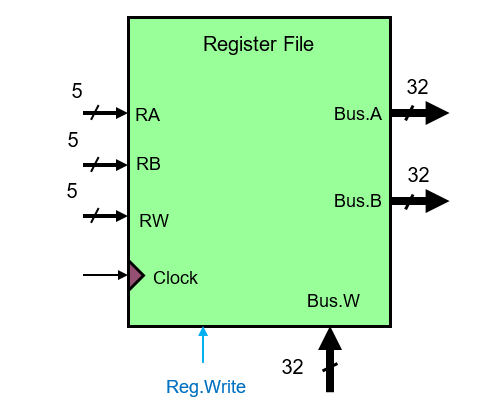
\includegraphics[width=16cm,height=10cm]{reg-file}%
		\captionof{figure}{32 $\times$ 32 Register File Interface}	
					\label{fig:fileInterface}%
	\end{center}
BusA and BusB are 32-bit data output busses for reading 2 registers. During read operation, the register file behaves as a combinational block and once the RA or RB have valid data, the content of the read register will appear on BusA or BusB after a certain access time.

RegWrite: control signal to enable/disable register writing operation. When RegWrite is 1, register write is enabled; otherwise, is disabled.
BusW has 32-bit data input bus for writing a register when RegWrite is 1
RA are 5-bits selection lines to select the register to be read on BusA.
RB are 5-bits selection lines to select the register to be read on BusB
and RW are 5-bits selection lines to select the register to be to be written with BusW.

The details of the designed 32 x 32 register file is shown in the following picture. In MIPS, register \$0 is always 0, so, register 0 is not used. In this picture, each of BusA and BusB is connected to 32 tri-state buffers. Each tri-state buffer is connected to one of the 32 registers. The tri-state buffers enable signals are driven by the outputs of two 5 to 32 decoders, one with Ra as input and the other with Rb as input, to select which register puts its value on the corresponding bus. To complete the writing operation, RW is connected as the input to another 5 to 32 decoder, and the outputs of this decoder provides the register selection signals for 31 registers (register 1 to 31). These register selection signals are ANDed with RegWrite to provide the writable enable signals for individual registers. 

	\begin{center}
		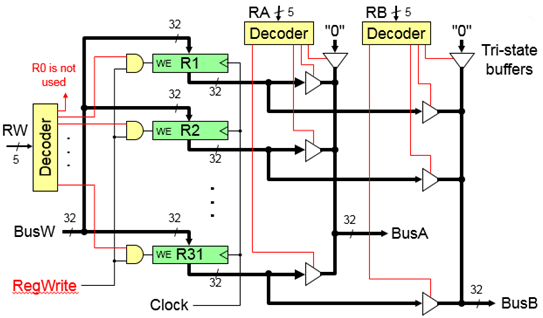
\includegraphics[width=16cm,height=8.5cm]{regFile}%
		\captionof{figure}{32 $\times$ 32 Register File Implementation with tri-state Buffers}	
					\label{fig:fileImplementation}%
	\end{center}
    \section{Register Design and Simulation in Logisim}
    \subsection*{Register 0 (\$0)}
    As already mentioned, in MIPS register 0 hereafter referred to as \$0 is always wired to 0 and cannot be written to. It must therefore be designed differently from the other registers. We use a tri-state buffer to control reading from \$0. \$0 is connected to bus A and bus B through a tri-state buffer. Wether \$0 puts its data on either of the buses depends on the control input to the tri-state buffer connecting it to that bus. A value of 1 will allow it to write to the bus (or to be read from) while a value of 0 puts it in the high impedance state.
    
      \begin{center}
		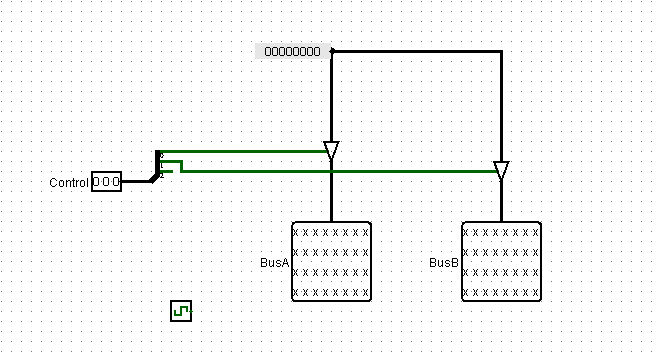
\includegraphics[width=16cm,height=6cm]{register-0}%
		\captionof{figure}{Register zero (\$0) with both tri-state buffers in high impedance state }	
					\label{reg-0}%
	\end{center}
    \subsection*{Register 1 to 31} 
    The other 31 registers are structurally the same. They differ from \$0 in that they can also be written to.  As in the case of \$0 we use two tri-state buffers to control the values read by bus A and bus B. The only new feature we need to introduce is a control for writing. It is prudent to use a synchronous design to avoid possible data corruption. We use a negative edge triggered circuit. A \textbf{write enable} control determines if the register can be written to or not at the falling edge of the  clock cycle.
      \begin{center}
		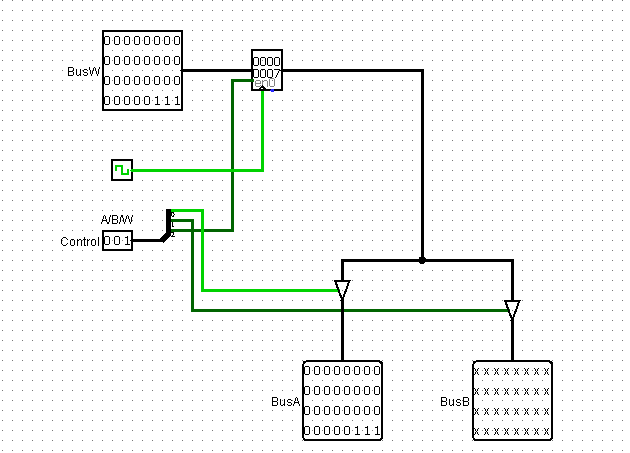
\includegraphics[width=16cm,height=10cm]{register}%
		\captionof{figure}{ 32 bit register whose data is available on Bus A}	
					\label{fig:reg-1-31}%
	\end{center}
	
     \subsection*{Zippers}
     This is a more nuanced aspect of our design but we present it here for the sake of completeness. Understanding how the zippers work is essential to understanding our organization of registers. The zippers are essentially used to bundle control wires. Each register needs 3 control signals one for reading to Bus A, another for reading to Bus B and another for write. There are two types of zippers we use: A $3 \times 4$ to $4 \times 3$ zipper takes in the 3 control lines of 4 different registers and distributes them to the "appropriate" registers.A $3 \times 16$ to $4 \times 12$ zipper performs a similar function.
      \begin{center}
		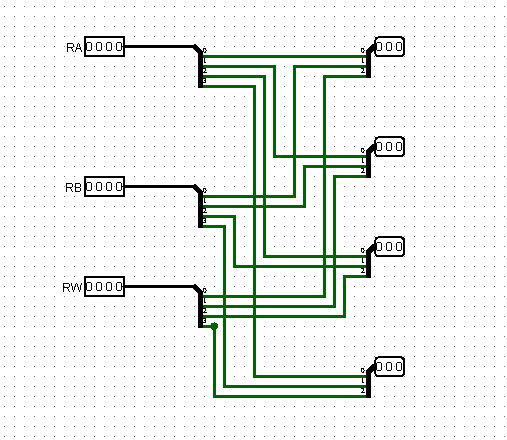
\includegraphics[width=15cm,height=10cm]{3x4zipper}%
		\captionof{figure}{A  $3 \times 4$ to $4 \times 3$ zipper}			\label{3x4zipper}%
	\end{center}
	      \begin{center}
		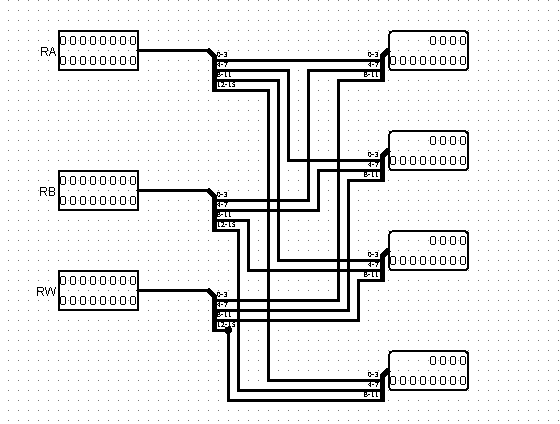
\includegraphics[width=15cm,height = 10cm]{3x16zipper}%
		\captionof{figure}{A  $3 \times 16$ to $4 \times 12$ zipper}			\label{3x16zipper}%
	\end{center}
    \subsection*{Register Cells}
    The register file is divided into 8 cells each having 4, 32 bit registers. A $3 \times 4$ to $4 \times 3 $ zipper is used to connect the control lines of each of the individual 4 registers as seen below.
    \begin{center}
		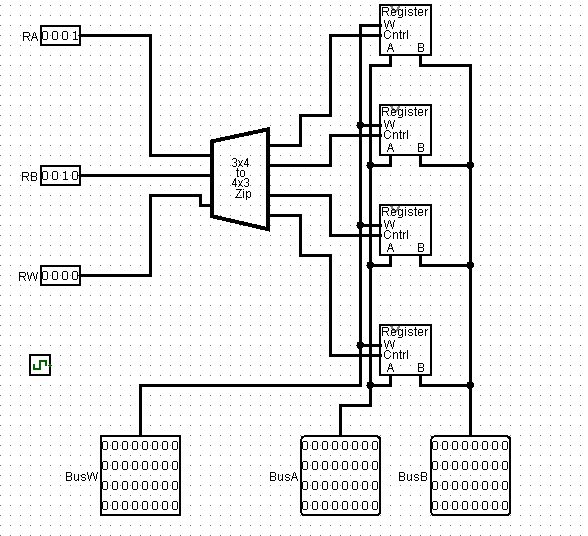
\includegraphics[width=18cm,height=14cm]{register-cell}%
		\captionof{figure}{A 4 $\times$ 8 register cell}	
					\label{reg-cell}%
	\end{center}
      \begin{center}
		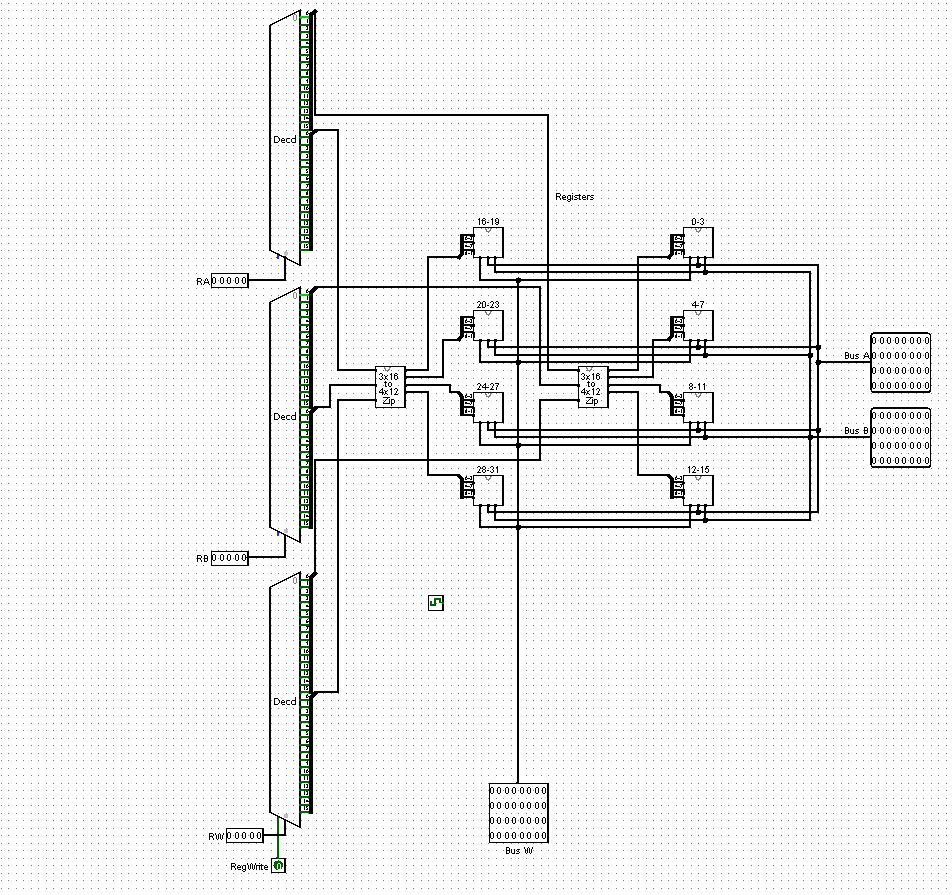
\includegraphics[width=16cm,height=14cm]{register-file}%
		\captionof{figure}{The 32 bit register file}	
					\label{reg-file}%
	\end{center}
	Finally we have the register file containing 32, 32 bit registers. The 32 registers are split into blocks of 8 cells. Each cell has 4 blocks.  There are 3, 32 bit address decoders for providing control signals for each of the registers. The top half of the bits (31 - 16) are passed to a separate $3 \times 16 $ to $4 \times 12$ zipper from the lower half (15 - 0) of the bits. The two $3 \times 16 $ to $4 \times 12)$ zippers are then connected to memory cells via $3 \times 4 $ to $4 \times 3)$ zippers.
   \mychapter{3}{ALU Design }
    In this section we design a 32 bit ALU to take care of integer arithmetic and other logical operations. The CPU is essentially a combinational circuit that receives two 32 bit inputs and produces a 32 bit result. Equivalently we may also view the process of designing a 32 bit ALU in the same way as designing and cascading 32 1 bit ALUs. Care however has to be taken in the design of the first and the last ALU as we will see shortly. 
\section{The 1 Bit ALU}
The 1 bit ALU takes in two 1 bit numbers A and B and performs arithmetic and logic operation on it. The operations performed by the ALU in Figure \ref{fig:alu1} below are \texttt{add, sub, or, and, xor}. Addition can be changed to subtraction by changing the \texttt{Sub} and \texttt{Cin} inputs from 0 to 1. Which output gets out of the ALU depends on the control signal placed on the select lines of the Multiplexer. Another thing worth noting is the \texttt{less} input. These are used in the execution of the \texttt{slt} and \texttt{slti} instructions. 

\section{The 32 bit ALU}
Both \texttt{slt} and \texttt{slti} instructions set the LSB of the ALU to 1 if ALU input A is less than ALU input B or 0 otherwise. The rest of the output bits up to the MSB are always 0 for this operation. For these instructions we subtract the first input operand from the second and check the MSB of the result. If it is  a 1, then it is negative and A is definitely less than B. But there is a problem here, we do the check on the MSB but what we want to set is the LSB. To get around this we connect the adder output of the last ALU to the less input of the first ALU.

Alas, the test of less than is a little more complicated than just described because of overflow. We will however not pursue this course any further since most programming languages do not check for overflow.
Notice that every time we want the ALU to subtract, we set both \texttt{Cin} and
 \texttt{Sub} to 1. For adds or logical operations, we want both control lines to be 0. We can therefore simplify control of the ALU by combining the \texttt{Cin} and  \texttt{Sub} to a single control line called \texttt{Sub}.
 
To further tailor the ALU to the MIPS instruction set, we must support
conditional branch instructions. These instructions branch either if two registers are equal or if they are unequal. The easiest way to test equality with the ALU is to subtract b from a and then test to see if the result is 0, since
$$(a - b= 0 \Longrightarrow a=b)$$
Thus, if we add hardware to test if the result is 0, we can test for equality. The
simplest way is to OR all the outputs together and then send that signal through an inverter:
$$Zero= (\overline{Result31 + Result30 + ...+Result2 + Result1 + Result0} )$$
Now that we have seen what is inside a 32-bit ALU, we will use the
universal symbol for a complete ALU as shown in \ref{fig:aluSym}
\begin{center}
		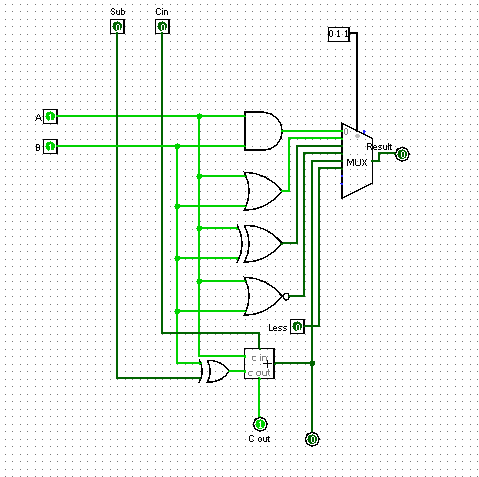
\includegraphics[width=16cm,height=10cm]{alu1}%
		\captionof{figure}{A 1 bit ALU perforrming  XOR in Logisim}	
					\label{fig:alu1}%
	\end{center}
The new 32 bit ALU is shown in Figure \ref{fig:alu32} below. Unfortunately  it's colossal size makes it hard  to provided a detailed view on paper.
\begin{center}
		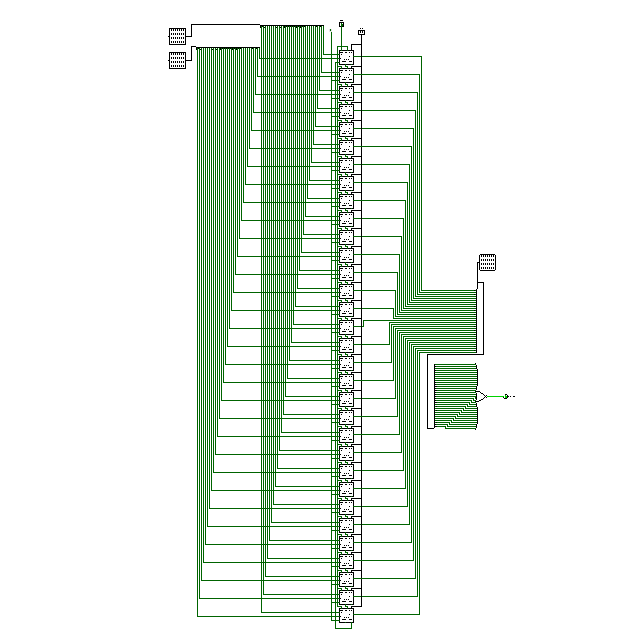
\includegraphics[width=16cm,height=14cm]{alu32}%
		\captionof{figure}{The Final 32 Bit ALU in Logisim}	
					\label{fig:alu32}%
		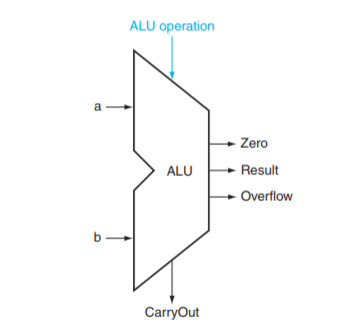
\includegraphics[scale=1]{aluSymbol}%
		\captionof{figure}{Generic ALU Symbol}	
					\label{fig:aluSym}%
	\end{center}
	
   \mychapter{4}{Datapath Design}
   \section{The Instruction Fetch Unit}
   All instructions require that the PC be incremented.
We will design a datapath which performs this function — the Instruction
Fetch Unit. Its operation is described by the following:

\begin{center}
{\hspace{25 mm} \large \texttt{mem[PC]} \hspace{25 mm} \text{ Fetch the instruction from memory}\\
 \texttt{ PC $\leftarrow$ PC + 4} \hspace{25 mm} \text{ Increment the PC}}
\end{center}
\begin{center}
		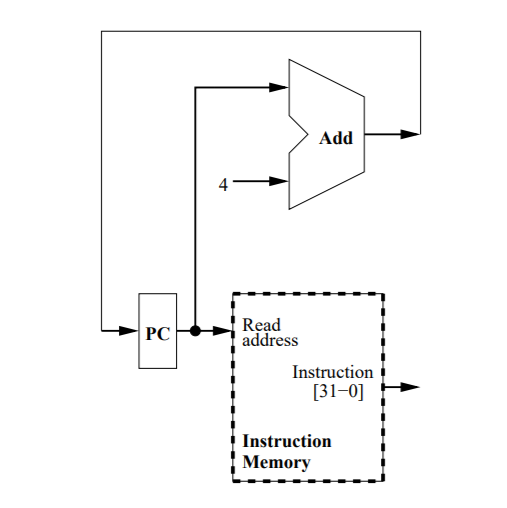
\includegraphics[width=10cm,height=8cm]{pc}%
		\captionof{figure}{Instruction Fetch Unit}	
					\label{fig:pc}%
	\end{center}
  This does not yet handle branches or jumps.
Since it is the same for all instructions, when describing individual
instructions this component will be omitted. PC is used as the instruction memory address to read instruction from the instruction memory, then PC is incremented by 4 to point to the next instruction to be executed. Since the instruction memory is aligned on 4-byte boundary, the least significant 2-bits of instruction addresses will always be 0. Thus, we can use 30-bit full-adder to update the most significant 30 bits of the PC.
\newpage
\section{Datapath for R-type instructions}
\begin{center}
\texttt{R[rd] $\longleftarrow$ R[rs] op R[rt] }
\end{center}
The datapath contains the 32 bit register file and and ALU capable
of performing all the required arithmetic and logic functions. The register file is read from and written to at the "same
time." This implies that the register’s memory elements must be
edge triggered, or are read and written on different clock phases, to
allow the arithmetic operation to complete before the data is written
in the register.
\begin{center}
		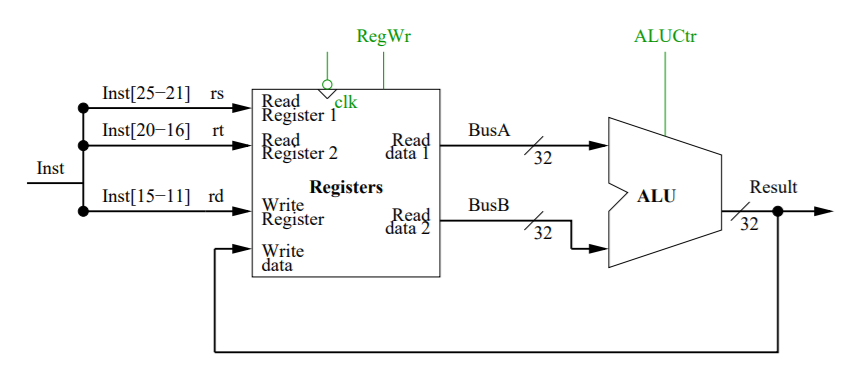
\includegraphics[width=18cm,height=8cm]{r-datapath}%
		\captionof{figure}{R-Type Instruction Datapath}	
					\label{fig:r-datapath}%
	\end{center}
	This datapath contains everything required to implement the required
instructions \texttt{add, sub, and, or, slt}. All that is required
is that the appropriate values be provided for the \texttt{ALUCtr} input for
the required operation.
The register operands in the instruction field determine the registers
which are read from and written to, and the \texttt{funct} field of the
instruction determine which particular ALU operation is executed.
\newpage
\section{Datapath for Immediate arithmetic and logical instructions}
The main difference between this and an r-type instruction is that
here one operand is taken from the instruction, and sign extended (for
signed data) or zero extended (for logical and unsigned operations.) We introduce a multiplexer with \texttt{ALUSrc} as control input to second ALU input. We also introduce a multiplexer with control \texttt{RegDest} for selecting the write address. In the case of I instruction it is from bits 20 to 16 but in immediate it is from 15 - 11.
\begin{center}
\texttt{R[rt] $\longleftarrow$ R[rs] op imm16}
\end{center}
\begin{center}
		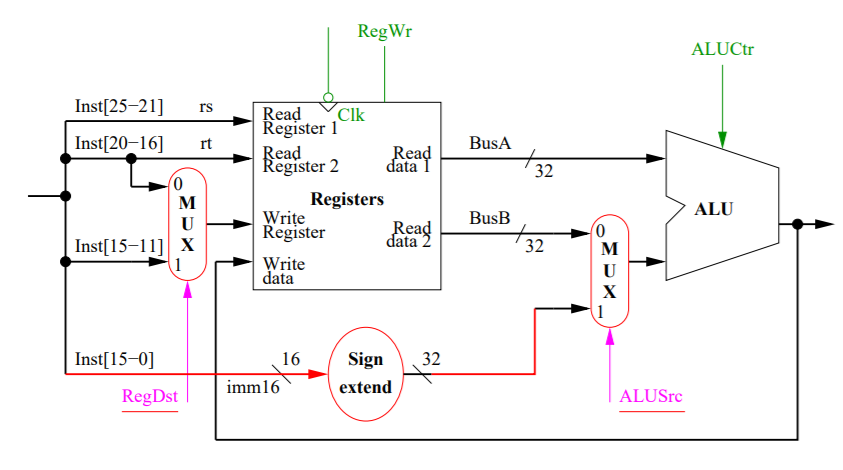
\includegraphics[width=18cm,height=12cm]{i-datapath}%
		\captionof{figure}{I-Type Instruction Datapath}	
					\label{fig:i-datapath}%
	\end{center}
	\newpage
\section{Datapath for the Load instruction}
\begin{center}
\texttt{lw rt, rs, imm16\\
Addr $\longleftarrow$ R[rs] +
SignExt(imm16)\\
R[rt] $\longleftarrow$ Mem[Addr]}
\end{center}
Both load and R type instructions can write to the register so we introduce a mux with control \texttt{MemtoReg} to select if the data written to the ALU comes from the data memory or from the ALU directly.
\begin{center}
		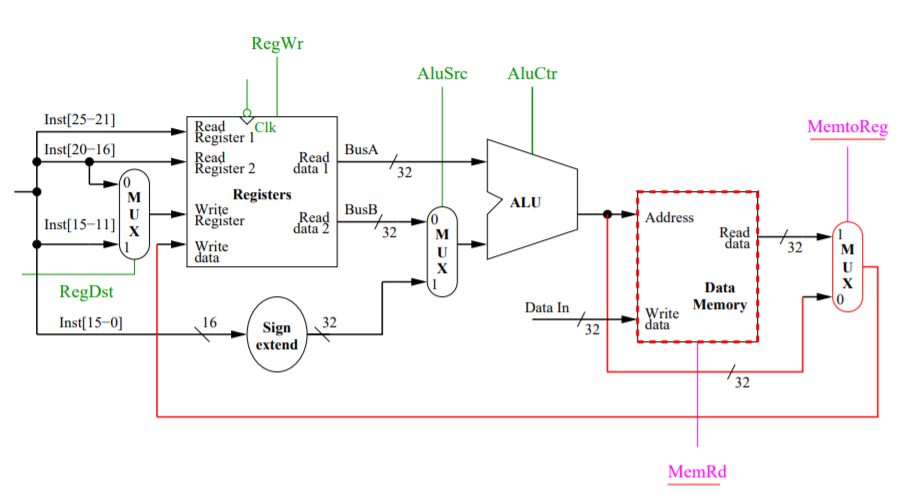
\includegraphics[width=18cm,height=12cm]{load-datapath}%
		\captionof{figure}{Load Instruction Datapath}	
					\label{fig:load-datapath}%
	\end{center}
	\newpage
\section{Datapath for the Store instruction}
\begin{center}
  \texttt{sw rt, rs, imm16\\
 Addr $\longleftarrow$ R[rs] +
SignExt(imm16)\\
 Mem[Addr]$\longleftarrow$ R[rt]}
\end{center}
\begin{center}
		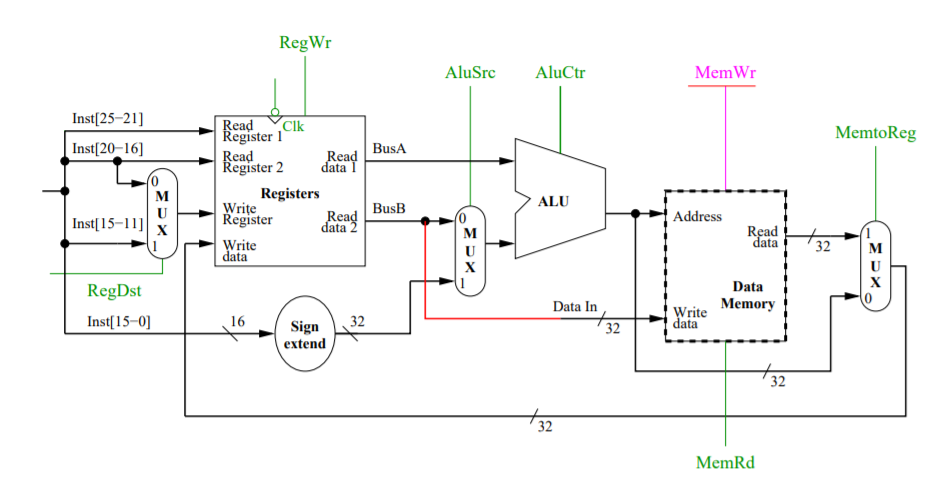
\includegraphics[width=18cm,height=12cm]{store-datapath}%
		\captionof{figure}{Store Instruction Datapath}	
					\label{fig:store-datapath}%
	\end{center}
	\newpage
\section{Datapath for the Branch and jump instruction}
\begin{center}
  \texttt{beq rt, rs, imm16\\
 Cond $\longleftarrow$ R[rs] - R[rt] \\
      if (Cond eq 0)\\
PC $\longleftarrow$ PC + 4 +
(SignExt(imm16) $\times$ 4)\\
 else PC$\longleftarrow$ PC + 4}
\end{center}
In the load and store instructions, the ALU was used to calculate
the address for data memory.
It is possible to do this for the branch instructions as well, but it
would require first performing the comparison using the ALU, and
then using the ALU to calculate the address.
This would require two clock periods, in order to sequence the operations
correctly.
A faster implementation would be to provide another adder to implement
the address calculation. This is what we will do.
\begin{center}
\texttt{j target\\
PC<31:2> $\longleftarrow$ PC<31:28>
concat target<25:0>}
\end{center}
\begin{adjustwidth}{-400pt}{-400pt}
\begin{center}
		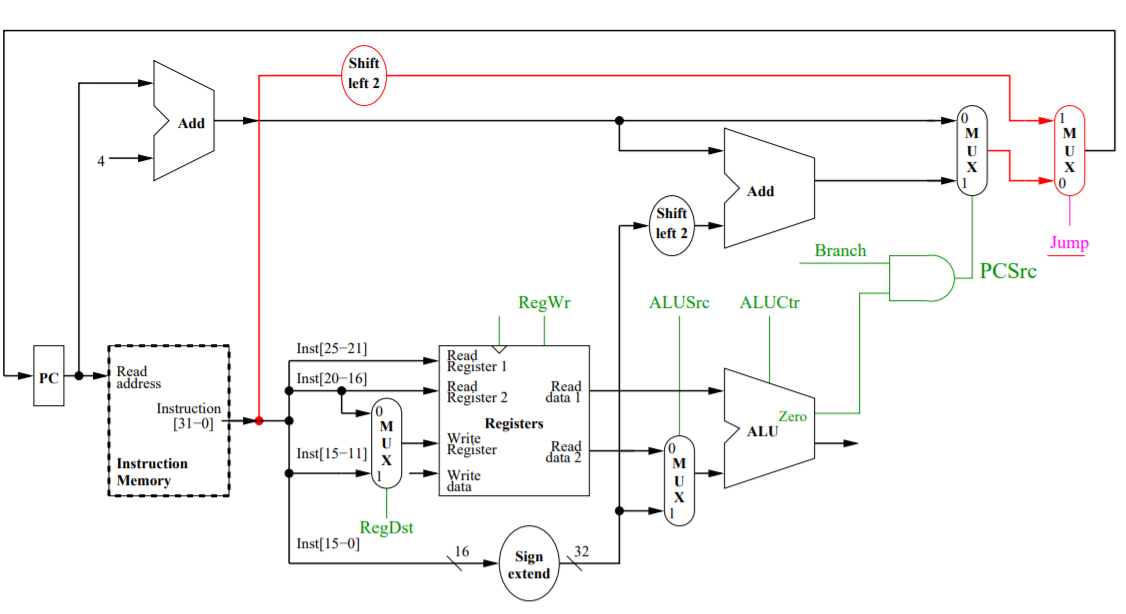
\includegraphics[width=20cm,height=13cm]{branch-jump-datapath}%
\end{center}
\end{adjustwidth}
\captionof{figure}{Branch and Jump Instruction Datapath}	
					\label{fig:branch-jump-datapath}%
\newpage
\section{Final Datapath}
We have incrementally built a data path for our processor at each stage we identified the required control signals.All that remains is to:
\begin{enumerate}
\item Combine the datapath elements
\item Design the appropriate control signals
\end{enumerate}
The required control signals are mainly the inputs for the multiplexers
and the signals required by the ALU.
The next figure shows, and the required control signals. The actual control logic is yet to be designed.
\begin{adjustwidth}{-400pt}{-400pt}
\begin{center}
		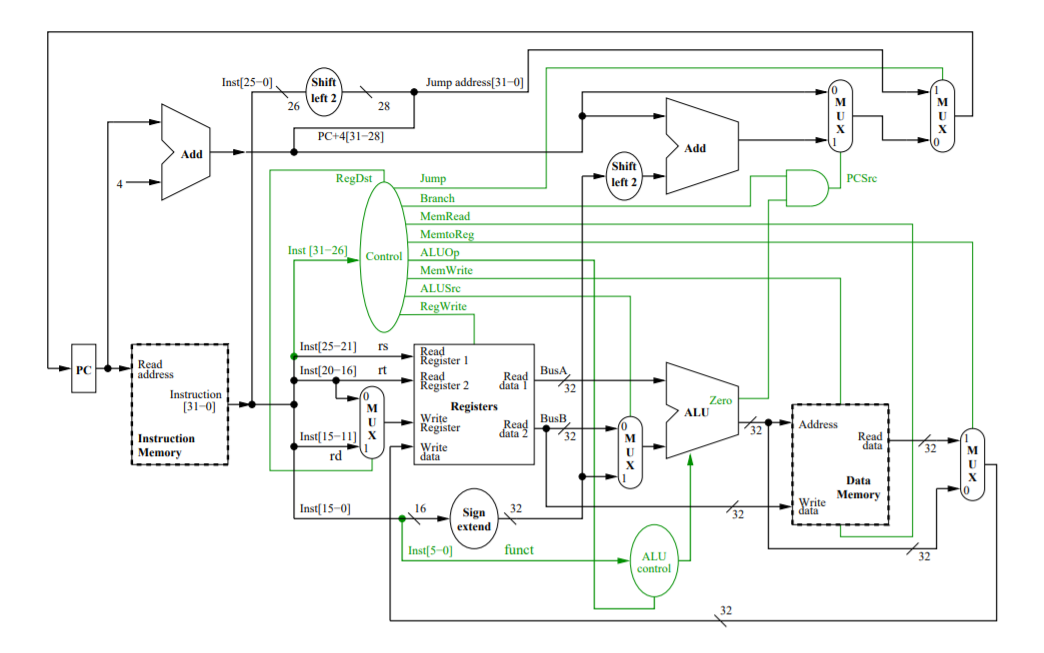
\includegraphics[width=23cm,height=15cm]{final-datapath}%
\end{center}
\end{adjustwidth}
\captionof{figure}{Complete Datapath with Required Control Logic }	
					\label{fig:final-datapath}%
   \mychapter{5}{Control Unit Design}
   The control provided here differs slightly from that shown in Figure \ref{fig:final-datapath} for design reasons. The reader should follow the continuation offered here without any hitch.We will have a main control unit and subcontrols for various units.
   \begin{center}
		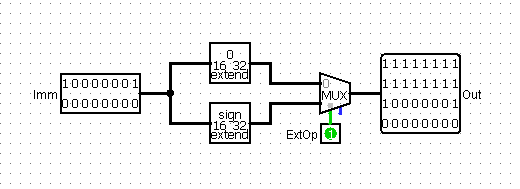
\includegraphics[width=9cm,height=4.5cm]{signExtender}%
		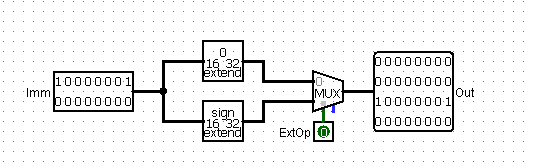
\includegraphics[width=9cm,height=4.5cm]{signExtender2}%
		\captionof{figure}{Sign Extension Unit Performing Sign Extension in the First Diagram and Zero Extension in the Second}	
					\label{fig:signExten}%
\end{center}
\section{Main Control Unit}
\begin{center}
\begin{longtable}{|l|l|l|l|l|l|c|c|c|c|c|c|}
\caption{Main Control Unit Truth Table} \label{tab:cu-table}\\
\hline
&R~~~~~&Jump&RegD&RegW&MemR&MemW&MTR&AluSrc&ExtOp&BNE&BEQ\\\hline
add&1&0&1&1&0&0&0&0&1&0&0\\\hline
sub&1&0&1&1&0&0&0&0&1&0&0\\\hline
and&1&0&1&1&0&0&0&0&1&0&0\\\hline
or&1&0&1&1&0&0&0&0&1&0&0\\\hline
xor&1&0&1&1&0&0&0&0&1&0&0\\\hline
slt&1&0&1&1&0&0&0&0&1&0&0\\\hline
addi&0&0&0&1&0&0&0&1&1&0&0\\\hline
ori&0&0&0&1&0&0&0&1&0&0&0\\\hline
xori&0&0&0&1&0&0&0&1&0&0&0\\\hline
andi&0&0&0&1&0&0&0&1&0&0&0\\\hline
slti&0&0&0&1&0&0&0&1&1&0&0\\\hline
lw&0&0&0&1&1&0&1&1&1&0&0\\\hline
sw&0&0&x&0&0&1&x&1&1&0&0\\\hline
beq&0&0&x&0&0&0&0&1&1&0&1\\\hline
bne&0&0&x&0&0&0&x&0&1&1&0\\\hline
j&0&1&x&0&0&0&x&x&x&0&0\\\hline
\end{longtable}
\end{center}
\begin{itemize}
\item R -R-Type
\item RegD - RegDest
\item RegW - RegWrite
\item MemR - MemRead
\item MemW - MemWrite
\item MTR - MemToReg
\end{itemize}
By now the truth table should be pretty intuitive. We can directly design the circuit with Sum of Products (POS). To avoid any esoteric bolean algebra we won't provide any optimization via Quin Mcklusckey or karnaugh Maps. We do this with little penalty. The Control Unit designed from SOP is shown in Figure \ref{fig:cu}.

Apart from generating codes for the various multiplexer selects, the control unit also produce a 4 bit \texttt{ALUOp} code to be used by the ALU control unit. To ease design, we will use a symmetric code so that the 4 bit \texttt{ALUOp} code generated for immediate instructions matches the 4 least significant bits of the function field of their R type counterparts. That being said, we have the following truth table for the \texttt{ALUOp} code output.

\begin{longtable}{|c|c|}
\caption{ALUOpcode Truth Table} \label{aluTable}\\
\hline
Instruction&Opcode\\\hline
addi&0000\\\hline
andi&0100\\\hline
ori&0101\\\hline
xori&0110\\\hline
slti&1010\\\hline
\end{longtable}
The \texttt{lw} and \texttt{sw} instructions require address calculation by the CPU and so they will share the same code as \texttt{addi}. \texttt{BNE} and \texttt{BEQ} on the other hand require subtraction in order to compare both numbers so they share the same code with \texttt{subi}. This is demonstrated in the main control unit by using an or gate to choose from one of these inputs. A priority encoder is used to assign the \texttt{ALUOpcode} to each instruction.
\begin{adjustwidth}{-400pt}{-400pt}
\begin{center}
		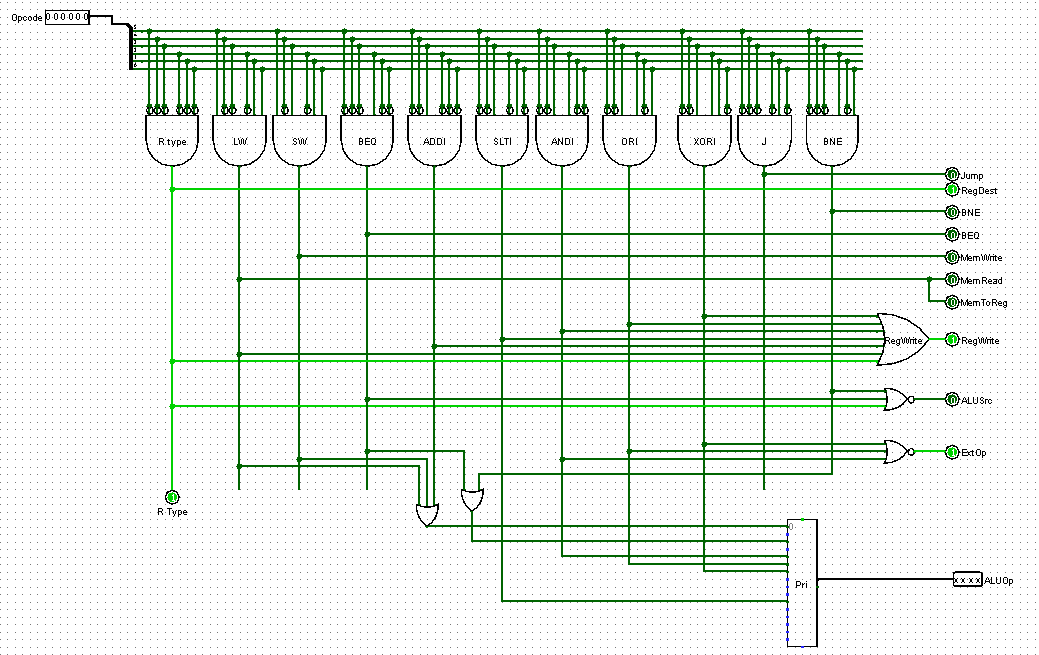
\includegraphics[width=21cm,height=18cm]{cu}%
\end{center}
\end{adjustwidth}
\captionof{figure}{Main Control Unit}	
					\label{fig:cu}%
\section{ALU Control}
\begin{center}
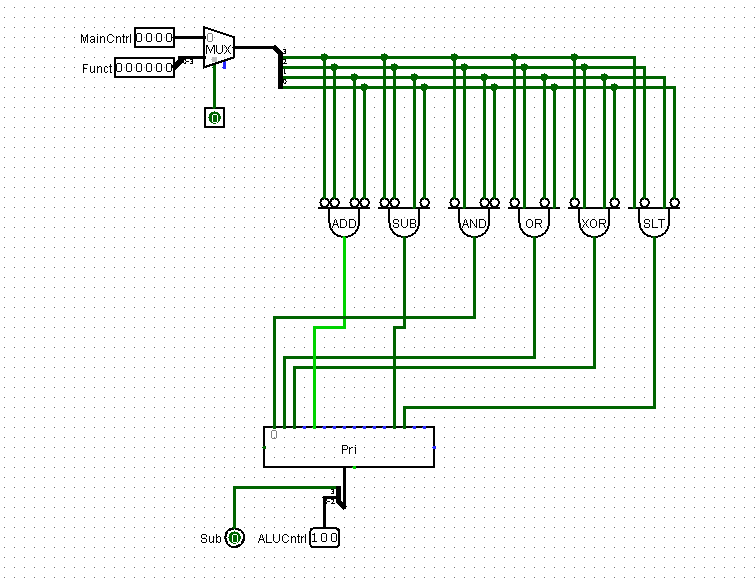
\includegraphics[width=15cm,height = 12cm]{aluControl}%
\caption{ALU Control}
\end{center}
The ALU control can have two sources of input. For I type instructions the input to the ALU are the opcodes describe in Table \ref{aluTable}. For the R type instructions, the input to the ALU consists of the 4 least significant bits of the function field. As already discussed, the 4 LSBs for the function field match exactly the 4 bits of the \texttt{ALUOpcode} for each complimentary R and I type instruction. The R output from the main control unit which determines if the instruction is an R type is connected to the select bit of the multiplexer. 

Finally, based on the operation from the ALU control we generate 3 output bits that can be used to select one of the 6 operations in our ALU.The bit 4 of the output is connected to the \texttt{sub} input of the ALU and therefore should only be 1 for operations needing subtraction i.e \texttt{sub} and \texttt{slt}. We generate the appropriate control codes using the priority encoder as follows.
\begin{longtable}{|c|c|c|}
\caption{\texttt{ALUCntrl} and \texttt{Sub} Outputs from Priority Encoder} \label{aluTab}\\\hline
Instruction&Sub&ALUCntrl\\\hline
And&0&000\\\hline
Or&0&001\\\hline
Xor&0&010\\\hline
Nor&0&011\\\hline
Add&0&100\\\hline
Sub&1&100\\\hline
Slt&1&101\\\hline
\end{longtable}
\section{PC Control}
\begin{center}
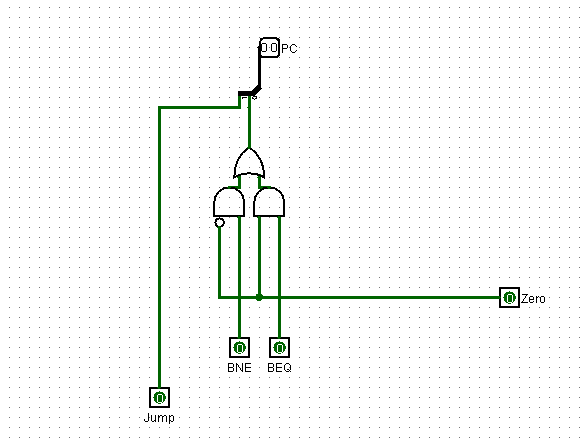
\includegraphics[width=15cm,height = 12cm]{pcControl}%
\caption{PC Control}
\end{center}
PC Control produces the output used to select how to increment the PC. Its output is a 2 bit field applied to a MUX that selects between jumping, branching and sequential operation.
\section{Final 32 bit CPU}
 \begin{adjustwidth}{-400pt}{-400pt}
\begin{center}
		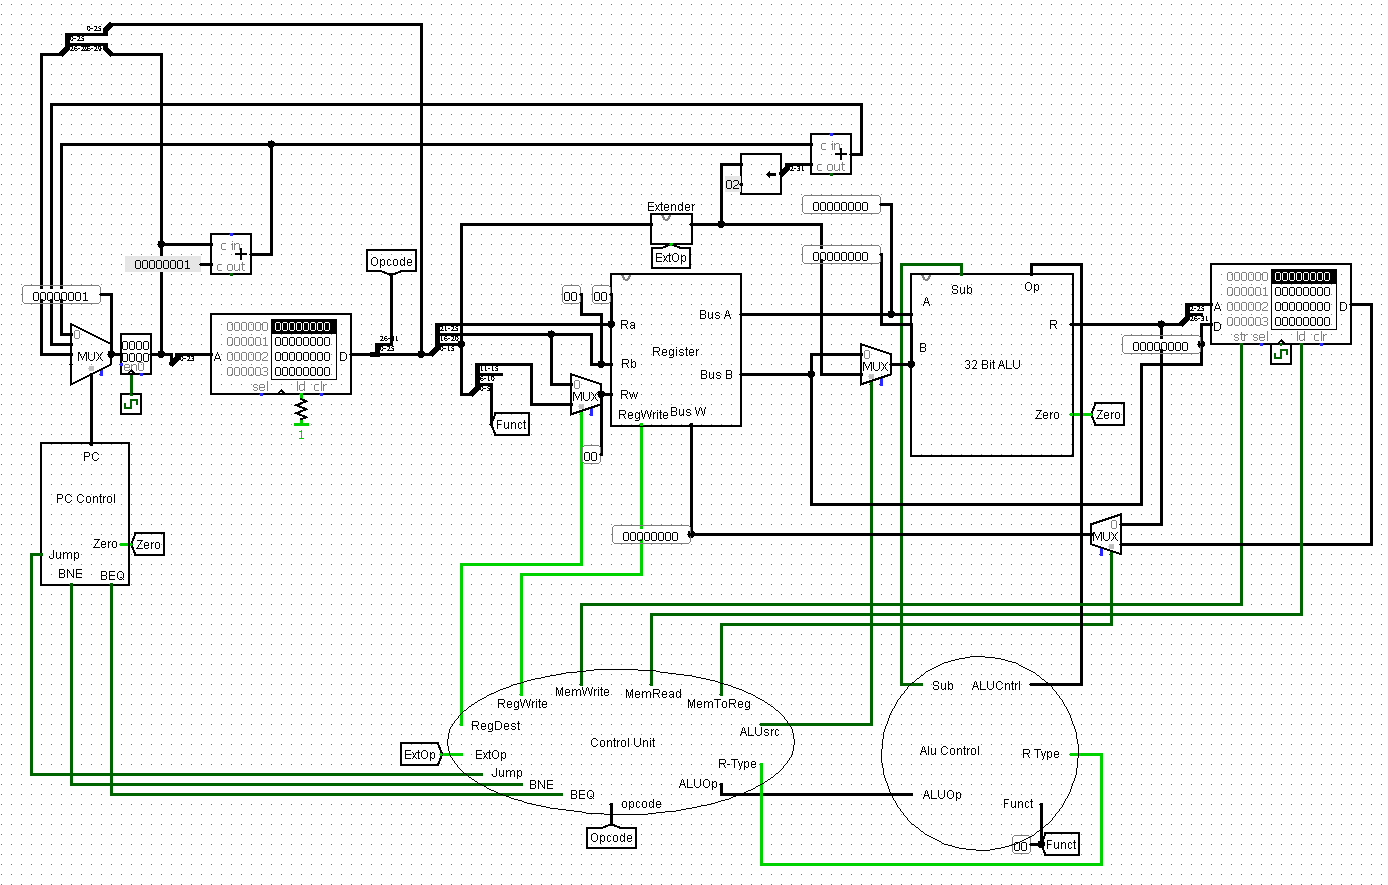
\includegraphics[width=21.5cm,height=17cm]{cpu}%
\end{center}
\end{adjustwidth}
\caption{Final 32 bit CPU}
\mychapter{6}{Testing}
In order to test our processor, we ran two test programs on the processor and rigorously followed through their execution. We hope we will be given time to do the demonstration in class. The two programs rigorously check the following eight instructions: and, or, sub, lw, sw,
slt, beq, add. 
\section{Test Program 1}
\subsection*{Assembly Language representation of test program 1}
\texttt{
sub r0,r0,r0    } \textsl{; set reg[0] to 0, use as base } \\
\texttt{lw  r1,0(r0)   } \textsl{ ; reg[1] <- mem[0] (= 1) } \\
\texttt{lw  r2,4(r0)}    \textsl{ ; reg[2] <- mem[4] (= A)  }\\
\texttt{lw  r3,8(r0)}     \textsl{; reg[3] <- mem[8] (= B) }\\
\texttt{sub r4,r4,r4}     \textsl{; reg[4] <- 0, running total}\\  
\texttt{add r4,r2,r4}     \textsl{; reg[4]+ = A  }\\
\texttt{slt r5,r2,r3}     \textsl{; reg[5] <- A < B } \\
\texttt{beq r5,r0,2 }     \textsl{; if reg[5] = FALSE, go forward 2 instructions } \\
\texttt{add r2,r1,r2}     \textsl{; A++ } \\
\texttt{beq r0,r0,-5}     \textsl{; go back 5 instructions }\\
\texttt{sw  r4,0(r0)}     \textsl{; mem[0] <- reg[4] } \\
\texttt{beq r0,r0,-1}     \textsl{; program is over, keep looping back to here }\\
\subsection*{Machine Language representation of test program 1 in Hex}
\texttt{
00000022
8c010000
8c020004
8c030008
00842022
00822020
0043282a
10a00002
00411020
1000fffb
ac040000
1000ffff}
\subsection*{Test Input 1}
\texttt{00000001
00000001
0000000a
}
\end{document}
